\documentclass[10pt,a4paper,oneside,fleqn]{report}
\usepackage{geometry}
\geometry{a4paper,left=20mm,right=20mm,top=1cm,bottom=2cm}
\usepackage[utf8]{inputenc}
%\usepackage{ngerman}
\usepackage{amsmath}                % brauche ich um dir Formel zu umrahmen.
\usepackage{amsfonts}                % brauche ich für die Mengensymbole
\usepackage{graphicx}
\setlength{\parindent}{0px}
\setlength{\mathindent}{10mm}
\usepackage{bbold}                    %brauche ich für die doppel Zahlen Darstellung (Einheitsmatrix z.B)
\usepackage[linktocpage={false}]{hyperref}


\usepackage{color}
\usepackage{titlesec} %sudo apt-get install texlive-latex-extra

\definecolor{darkblue}{rgb}{0.1,0.1,0.55}
\definecolor{darkred}{rgb}{0.55,0.2,0.2}

\titleformat{\chapter}[display]{\color{darkred}\normalfont\huge\bfseries}{\chaptertitlename\
\thechapter}{20pt}{\Huge}

\titleformat{\section}{\color{darkblue}\normalfont\Large\bfseries}{\thesection}{1em}{}
\titleformat{\subsection}{\color{darkblue}\normalfont\Large\bfseries}{\thesection}{1em}{}

% Notiz Box
\usepackage{fancybox}
\newcommand{\notiz}[1]{\vspace{5mm}\ovalbox{\begin{minipage}{1\textwidth}#1\end{minipage}}\vspace{5mm}}

\usepackage{cancel}


%\includegraphics[width=0.75\textwidth]{thepic.png}

\begin{document}
\tableofcontents
\setcounter{chapter}{11}
\chapter{Magnetismus}

Die Magnetisierung \(\vec M\) ist das magnetische Moment pro Volumen. \(\vec M = n\vec\mu\) ; \(\mu\) ist mittleres Dipolmoment.


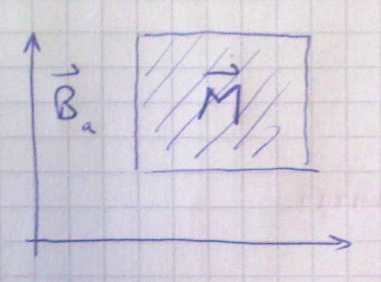
\includegraphics[width=0.75\textwidth]{kap12_01.png}


Magnetische Suszeptibilität: \([\chi]\) Tensor

\[[\chi]\equiv \chi = \frac{\vec M}{\vec H} = \mu_0\frac{\vec M}{\vec B} \]

Skalar (Vereinfacht) \(\chi= \frac{M}{H}\); \(\chi < 0 \): diamagnetische festkörper; \(\chi>0\): paramaggnetische Festkörper

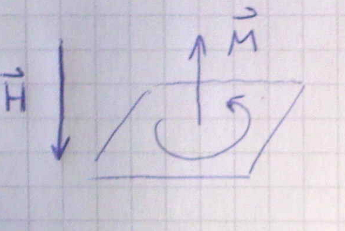
\includegraphics[width=0.75\textwidth]{kap12_02.png}


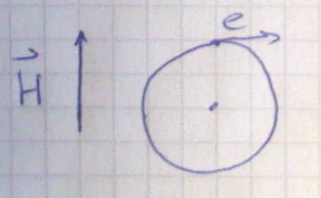
\includegraphics[width=0.75\textwidth]{kap12_03.png}


Lenz-Regel \(I \propto \frac{d\phi}{dt}\)

\section{Diamagnetismus}

Diamagnetismus ist eine Schwächung des äußeren Feldes. Klassische (Langevin) und quantenmechanische Behandlung. Beide kommen zu gleichen Resultaten. 




\[\left.\chi_d\right|_{\text{Atome}}\propto 10^{-6}\text{ bis }10^{-7}\]

\[\left.\chi_a\right|_{\text{Atome}} = -\frac{h\mu_0 e^2}{6m_e}Z \langle r^2\rangle \]

mit \(Z\) Elektronenzahl und \(\langle r^2\rangle  \) mittlerer abstandsquadrat der e-nen

\subsection{Diamagnetismus freier Elektronen: Landau-Diamagnetismus}

1930 Landau-Quantisierung \(\frac{\hbar(k^2_x+k^2_y)}{2m_e} = (l+\frac{1}{2})\hbar\omega_c\); \(l=0,1,2,3...\) B-Feld in z-Richtung.

mit \(\chi = -\frac{\partial^2 F}{\partial H^2}\)

\[F = k_B T ln\sum_{\text{alle Zustände}}e^{-\frac{iE}{k_B T}}\]

\[\left.\chi_d\right|_{\text{Landau}}= -\frac{1}{3}\mu_B^2\mu_0 D(E_F) =-\frac{1}{3}\mu_B^2\mu_0 \frac{3}{2}\frac{n}{E_F} = -\frac{n}{2E_F}\mu_0\mu_B^2 \propto 2\cdot 10^{-7} \]

mit dem Borsches Magneton \( \mu_B=\frac{e\hbar}{2m_e} \) und Zustandsdichte \(D(E_F) \)


\section{Paramagnetismus}

Paramagnetismus freier e-nen ist allgemein bekannt als Paulische Spin Suszeptibilität.

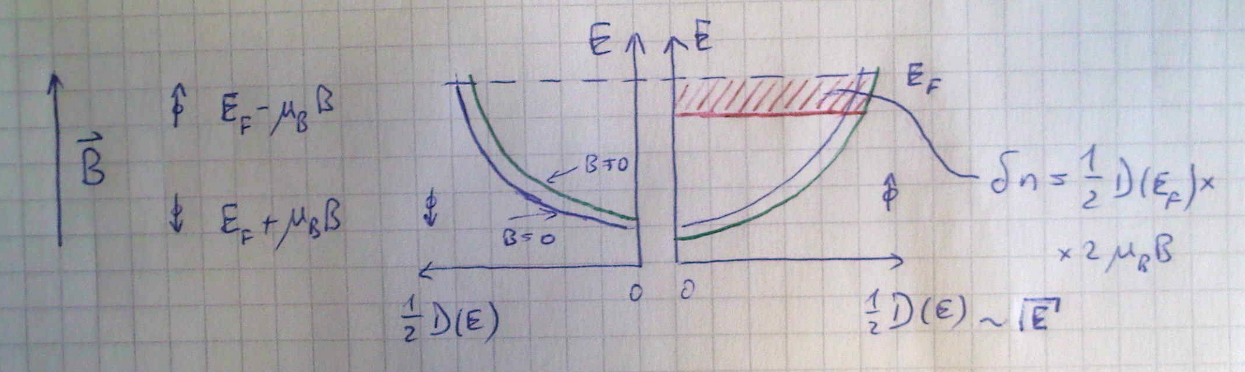
\includegraphics[width=0.75\textwidth]{kap12_04.png}

Roter Bereich \(\delta n\) kommt dazu, es gibt insgesammt mehr Elektronen

\[\delta n = \frac{1}{2}D(E_F) 2\mu_BB\]

\[M = \delta n \mu_B = \mu_B^2 B D(E_F)\]

\[\left.\chi_P\right|_{\text{Pauli}} =\mu_B\frac{M}{B} = \mu_0\mu_B^2 d(E_F) = \left.-3\chi_d\right|_{\text{Landauu}}\]

\[\boxed{ \left.\chi_P\right|_{\text{Landau}} = \left.-\frac{1}{3} \chi_d\right|_{\text{Pauli}} }\]


\subsection{Paramagnetismus von Ionen}

Aus der Atomphysik: \( \vec \mu = -g\mu_B\vec J'\) mit \(g\) Lande-Faktor \(\vec J'\hbar \vec J\) Gesamtdrehimpuls des Atoms

\[\hat J = \hat L + \hat S\]

\[g = 1 + \frac{J(J+1)+S(S+1)-L(L+1)}{2J(J+1)}\]

\(L\)-Bahndrehimpulsquantenzahl und \(S\)-Spinquantenzahl

Quantentheorie ( nur für Zwei-Niveau-Spinsystem)


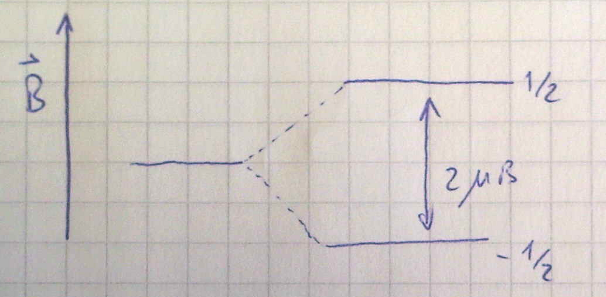
\includegraphics[width=0.75\textwidth]{kap12_05.png}

\[V = -\vec \mu\vec B = \underbrace{m_J g\mu_B}_{\mu} B\]

mit \(m_J=\pm\frac{1}{2}\); \(g=2\); \(V = \pm\mu_B B\)


Im Gleichgewicht für \(T\neq 0\); Faktor \(x=\frac{\mu B}{k_BT}\)

\[\frac{n_\uparrow}{n} = \frac{e^x}{e^x+e^{-x}}\]

\[\frac{n_\downarrow}{n} = \frac{e^{-x}}{e^x+e^{-x}}\]

Magnetisierung \(M=(n_\uparrow - n_\downarrow)\mu = n\mu tanh(x)\)

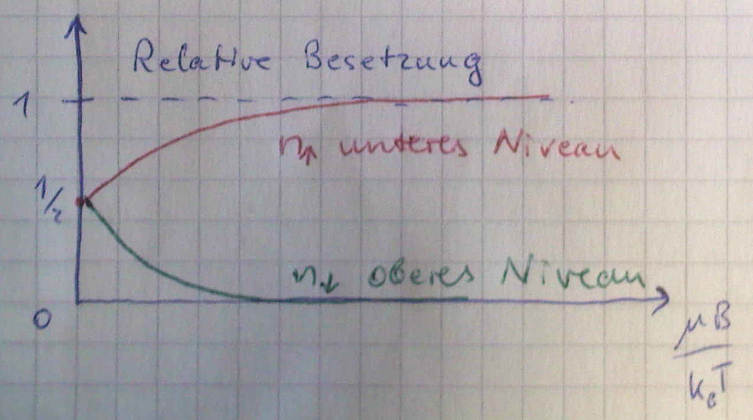
\includegraphics[width=0.75\textwidth]{kap12_06.png}

für \(x<<1\) (hohe T) \(tanh(x)\propto x\)

\[M\approx n\mu \frac{\mu B}{k_B T}\]

Curie-Gesetz:
\[\chi_{pa}\approx \frac{n\mu^2}{k_BT}\mu_0\approx \frac{1}{T}\]
Ein Atom mit Gesamtdrehimpulsquantenzahl J besitzt in einem Magnetfeld (2J+1) äquidistante Energieniveaus

\[M = ngJ\mu_B B_J(x)\]

mit \( B_J(x) \) Brillouin-Funktion für \(x<<1\)

\[\chi_{pi} = \mu_0\frac{\mu}{B} = n J(J+1)\frac{g^2\mu_B}{3k_BT}\propto\frac{C}{T}\]

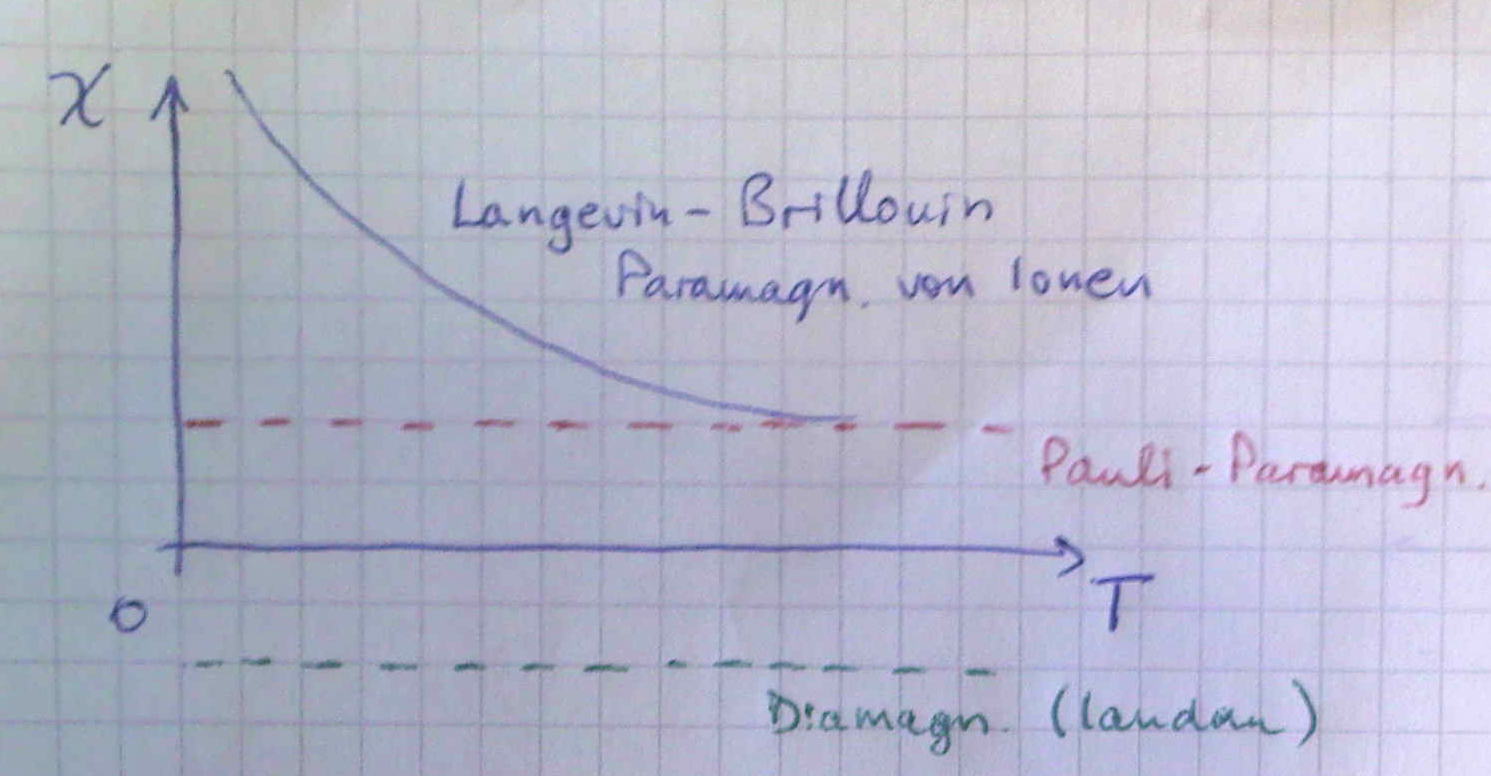
\includegraphics[width=0.75\textwidth]{kap12_07.png}

\section{Kühlung durch adiabatische Entmagnetisierung}

von Debye 1926 vorgeschlagen und 7 Jahre später realisiert.

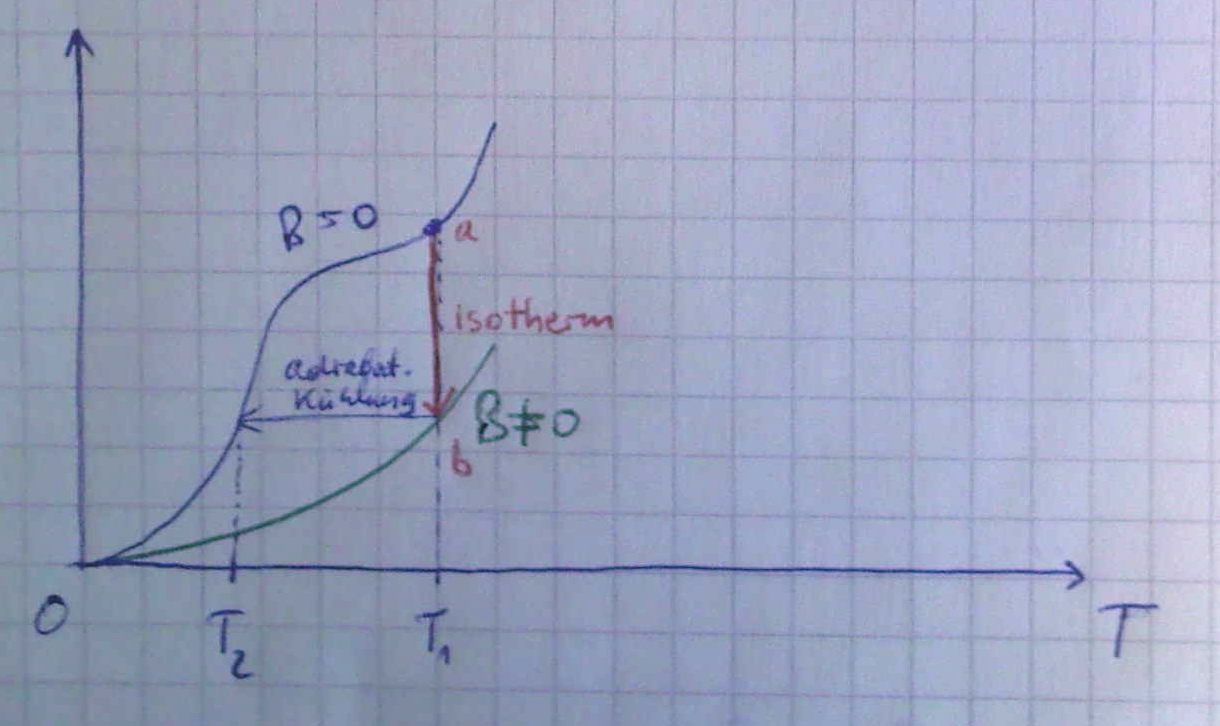
\includegraphics[width=0.75\textwidth]{kap12_08.png}

a - gute Wärmekontakt bis \(mK\)
b - Probe von Umgebung isoliert \(\approx 10 \mu K\) Bei Cu Kernentmagnetisierung


\end{document}
